\documentclass[12pt]{article}
\usepackage{fullpage, amsmath, amssymb, amsthm, amscd, setspace, bm, graphicx, indentfirst, multirow, tikz, enumerate}
\usepackage{adjustbox,amsfonts,array,graphicx,booktabs,tabularx,multirow,multicol,stmaryrd, tabu}
\usepackage[utf8]{inputenc}
\usetikzlibrary{arrows.meta}
\title{Math 412, Fall 2023 -- Homework 2}
\date{}
\setlength{\parskip}{0.5cm}
\setlength{\parindent}{0cm}

\newtheorem{theorem}{Theorem}[section]
\newtheorem{definition}[theorem]{Definition}
\newtheorem{lemma}[theorem]{Lemma}
\newtheorem{proposition}[theorem]{Proposition}
\newtheorem{corollary}[theorem]{Corollary}
\newtheorem{remark}[theorem]{Remark}
\newtheorem{example}[theorem]{Example}

\newcommand{\Z}{\mathbb{Z}}
\newcommand{\R}{\mathbb{R}}
\newcommand{\Q}{\mathbb{Q}}
\newcommand{\C}{\mathbb{C}}
\newcommand{\ba}{\overline}
\newcommand{\Hom}{\text{Hom}}
\newcommand{\End}{\text{End}}
\begin{document} \maketitle
\vspace{-80pt}

\textbf{Due:} Wednesday, September 6th, at 9:00AM via Gradescope

\textbf{Instructions:} Students taking the course for three credit hours (undergraduates, most graduate
students) should choose four of the following five problems to solve and turn in--if you do all five, only the first four will be graded. Graduate students
taking the course for four credits should solve all five. Problems that use the word ``describe”,
``determine”, ``show", or ``prove" require proof for all claims.

\begin{enumerate}

\item[1.] Recall that $K_n$ denotes the complete graph on $n$ vertices. Prove or disprove.

\begin{enumerate}
    \item[a.] For every $e,f\in E(K_n)$, $(K_n\setminus e) \cong (K_n\setminus f)$.
    \item[b.] For every $e_1,e_2,f_1,f_2\in E(K_n)$ such that $e_1\ne e_2$ and $f_1\ne f_2$, \[((K_n\setminus e_1)\setminus e_2) \cong ((K_n\setminus f_1)\setminus f_2).\]
\end{enumerate}

\item[2.] Let $G$ be a graph, let $e$ be an edge of $G$ and let $W$ be a closed walk in $G$ such that $e$ is in $W$ an odd number of times. Prove that $W$ contains a cycle that contains the edge $e$. 

\item[3.] Determine for which values $m$ and $n$ the complete bipartite graph $K_{m,n}$ has an Eulerian circuit.

\item[4.] Prove that a loopless graph $G$ is bipartite if and only if every subgraph $H$ of $G$ has an independent set of size at least $|V(H)|/2$.

\item[5.] Two Eulerian circuits in a graph $G$ are \emph{equivalent} if they have the same cyclic sequence of edges or if one cyclic sequence is the reverse of the other. For example,
    \begin{align*}
        (v_0, e_1, v_1, e_2, v_3, e_3, v_0) \hspace{15pt} \text{and} \hspace{15pt}
        (v_1, e_2, v_3, e_3, v_0, e_1, v_1) \hspace{15pt} \text{and} \hspace{15pt}
        (v_0, e_3, v_3, e_2, v_1, e_1, v_0)
    \end{align*}
    are all equivalent Eulerian circuits. How many equivalence classes of Eulerian circuits are there for the following graph $G$? This problem does \emph{not} require proof; however, you \emph{do} need to write down an Eulerian circuit for each equivalence class.
    \begin{center}
        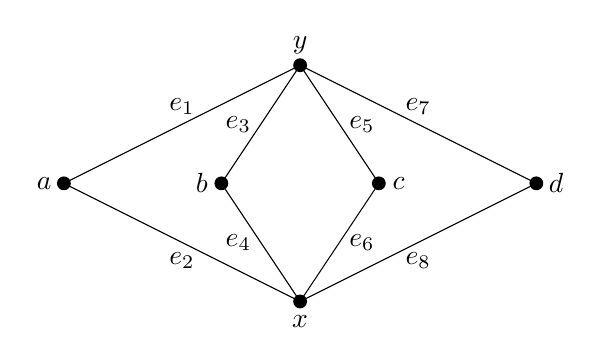
\begin{tikzpicture}
            \draw [line width=0.25mm, fill=black] (0,0) circle (0.75mm);
            \draw [line width=0.25mm, fill=black] (0,3) circle (0.75mm);
            \draw [line width=0.25mm, fill=black] (-3,1.5) circle (0.75mm);
            \draw [line width=0.25mm, fill=black] (-1,1.5) circle (0.75mm);
            \draw [line width=0.25mm, fill=black] (1,1.5) circle (0.75mm);
            \draw [line width=0.25mm, fill=black] (3,1.5) circle (0.75mm);
            \draw (0,0) to node[midway,below]{$e_2$} (-3,1.5);
            \draw (-3,1.5) to node[midway,above]{$e_1$} (0,3);
            \draw (0,0) to node[midway,left]{$e_4$} (-1,1.5);
            \draw (-1,1.5) to node[midway,left]{$e_3$} (0,3);
            \draw (0,0) to node[midway,right]{$e_6$} (1,1.5);
            \draw (1,1.5) to node[midway,right]{$e_5$} (0,3);
            \draw (0,0) to node[midway,below]{$e_8$} (3,1.5);
            \draw (3,1.5) to node[midway,above]{$e_7$} (0,3);
            \node at (0,-0.25) {$x$};
            \node at (0,3.25) {$y$};
            \node at (-3.25,1.5) {$a$};
            \node at (-1.25,1.5) {$b$};
            \node at (1.25,1.5) {$c$};
            \node at (3.25,1.5) {$d$};
        \end{tikzpicture}
    \end{center}


\end{enumerate}


\end{document}
